%!LW recipe=latexmk-xelatex-clean
% !TeX program = xelatex
% !TEX TS-program = xelatex
% !TeX root = week1_ppt_beamer_microgrid_intro.tex
\documentclass[aspectratio=169,10pt]{ctexbeamer}

\usetheme{Madrid}
\usecolortheme{seahorse}
\setbeamertemplate{navigation symbols}{}
\setbeamertemplate{footline}[frame number]

\usepackage{amsmath,amssymb,booktabs,array}
\usepackage{tikz}
\usetikzlibrary{arrows.meta,positioning,shapes.geometric,fit,calc}
\usepackage{listings}
\usepackage{xcolor}
\usepackage{hyperref}

\definecolor{codebg}{RGB}{248,248,248}
\definecolor{darkblue}{RGB}{0,65,120}
\definecolor{darkgreen}{RGB}{0,105,70}
\definecolor{warnorange}{RGB}{190,110,0}

\hypersetup{colorlinks=true,linkcolor=darkblue,urlcolor=darkblue}

\lstdefinestyle{pythonstyle}{
    language=Python,
    basicstyle=\ttfamily\scriptsize,
    keywordstyle=\color{darkblue}\bfseries,
    commentstyle=\color{darkgreen},
    stringstyle=\color{warnorange},
    showstringspaces=false,
    columns=fullflexible,
    backgroundcolor=\color{codebg},
    frame=single,
    rulecolor=\color{black!15},
    breaklines=true
}
\lstset{style=pythonstyle}

\newcommand{\code}[1]{\texttt{#1}}
\newcommand{\checkitem}{\textcolor{darkgreen}{\Large$\checkmark$}\;}
\newcommand{\warnitem}{\textcolor{warnorange}{\Large$\triangle$}\;}

\title[Week 1: Microgrid + pandapower]{Week 1: Microgrid Security Prediction and First pandapower Model}
\subtitle{Physics-informed AI for Three-phase Unbalanced N-1 Security Screening}
\author{ECE Course - Research Tutorial}
\institute{Microgrid 3-phase Security AI Project}
\date{2026}

\begin{document}

% ----------------------------------------------------------------------
\begin{frame}
  \titlepage
  \vspace{-0.8em}
  \begin{center}
    \small 本周关键词: microgrid, static security, pandapower, power flow, validation
  \end{center}
\end{frame}

% ----------------------------------------------------------------------
\begin{frame}{本周学习目标}
\begin{columns}[T]
\column{0.52\textwidth}
学生完成 Week 1 后应能:
\begin{itemize}
  \item 解释微电网安全预测的科研故事线;
  \item 识别 pandapower 中的 bus, line, trafo, load, sgen, storage, ext\_grid;
  \item 搭建一个小型 microgrid-like radial feeder;
  \item 运行平衡 AC 潮流 \code{pp.runpp(net)};
  \item 读取 \code{net.res\_bus}, \code{net.res\_line}, \code{net.res\_trafo};
  \item 用基本物理检查验证潮流结果。
\end{itemize}
\column{0.42\textwidth}
\begin{block}{本周边界}
本周先用平衡模型建立仿真。Week 2 再进入 \code{runpp\_3ph}, \code{asymmetric\_load}, \code{asymmetric\_sgen} 和三相结果表。
\end{block}
\begin{alertblock}{安全预测关注点}
不是只追求 accuracy, 而是降低 false negative: 不要把危险场景误判为安全。
\end{alertblock}
\end{columns}
\end{frame}

% ----------------------------------------------------------------------
\begin{frame}{八周项目路线图}
\centering
\begin{tikzpicture}[node distance=0.65cm and 0.65cm, every node/.style={font=\scriptsize}]
\tikzset{box/.style={draw, rounded corners, align=center, minimum width=2.15cm, minimum height=0.72cm, fill=blue!6}}
\tikzset{arrow/.style={-{Latex[length=2mm]}, thick}}
\node[box] (w1) {Week 1\\故事线 + pandapower};
\node[box, right=of w1] (w2) {Week 2\\三相不平衡潮流};
\node[box, right=of w2] (w3) {Week 3\\场景生成};
\node[box, right=of w3] (w4) {Week 4\\N-1 标签};
\node[box, below=of w1] (w5) {Week 5\\ML baseline};
\node[box, right=of w5] (w6) {Week 6\\Physics-informed MLP};
\node[box, right=of w6] (w7) {Week 7\\Phase-aware GNN};
\node[box, right=of w7] (w8) {Week 8\\论文和展示};
\draw[arrow] (w1) -- (w2);
\draw[arrow] (w2) -- (w3);
\draw[arrow] (w3) -- (w4);
\draw[arrow] (w4) -- ++(0,-0.58) -| (w5);
\draw[arrow] (w5) -- (w6);
\draw[arrow] (w6) -- (w7);
\draw[arrow] (w7) -- (w8);
\end{tikzpicture}
\vspace{0.8em}
\begin{block}{最终研究原型}
用 pandapower 三相潮流和 N-1 扫描生成标签, 用 AI 模型快速预测 violation risk, 再把高风险 contingency 交给精确潮流验证。
\end{block}
\end{frame}

% ----------------------------------------------------------------------
\begin{frame}{科研故事线: 为什么是 microgrid?}
\begin{columns}[T]
\column{0.54\textwidth}
\begin{itemize}
  \item 微电网由本地负荷、分布式电源、储能和控制边界组成;
  \item 它可以并网运行, 也可以在故障或调度需要时孤岛运行;
  \item 关键负荷需要更高供电可靠性;
  \item 高比例 PV, EV 和 BESS 让运行状态更快变化;
  \item 运维人员需要快速判断: 当前状态能否承受某个设备退出?
\end{itemize}
\column{0.42\textwidth}
\begin{block}{工程叙事}
传统配电网分析常看单个工况; 微电网需要看大量 operating scenarios 和 contingency。AI 的角色是 fast screening。
\end{block}
\footnotesize DOE 的 microgrid fact sheet 强调了清晰电气边界、可控实体、并网/孤岛运行等定义要素。\footnote{DOE Grid Deployment Office, Microgrid Overview Fact Sheet, 2024.}
\end{columns}
\end{frame}

% ----------------------------------------------------------------------
\begin{frame}{微电网示意图}
\centering
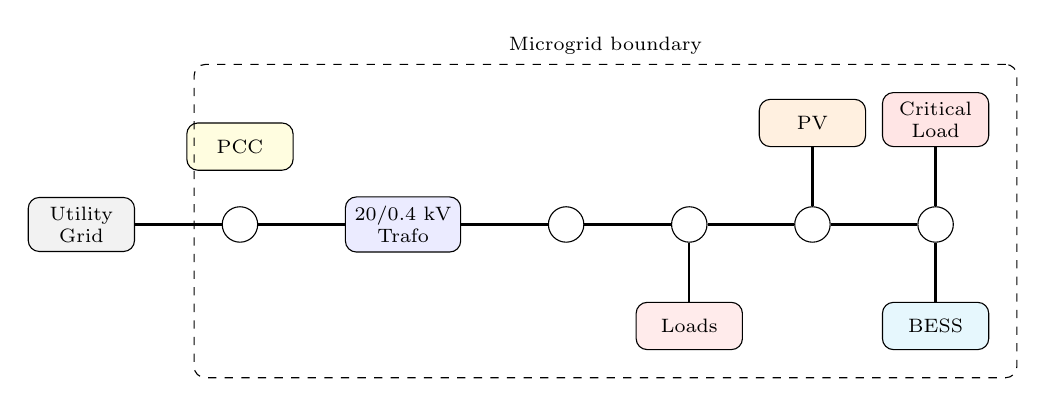
\begin{tikzpicture}[node distance=1.0cm and 1.1cm, every node/.style={font=\scriptsize}]
\tikzset{bus/.style={draw, circle, minimum size=0.45cm, fill=white}}
\tikzset{dev/.style={draw, rounded corners, align=center, minimum width=1.35cm, minimum height=0.6cm, fill=green!7}}
\tikzset{line/.style={thick}}
\node[dev, fill=gray!10] (grid) {Utility\\Grid};
\node[bus, right=of grid] (pcc) {};
\node[dev, above=0.45cm of pcc, fill=yellow!12] {PCC};
\node[dev, right=of pcc, fill=blue!8] (trafo) {20/0.4 kV\\Trafo};
\node[bus, right=of trafo] (b0) {};
\node[bus, right=of b0] (b1) {};
\node[bus, right=of b1] (b2) {};
\node[bus, right=of b2] (b3) {};
\node[dev, above=0.75cm of b2, fill=orange!12] (pv) {PV};
\node[dev, below=0.75cm of b3, fill=cyan!10] (bess) {BESS};
\node[dev, below=0.75cm of b1, fill=red!8] (load) {Loads};
\node[dev, above=0.75cm of b3, fill=red!10] (crit) {Critical\\Load};
\draw[line] (grid) -- (pcc) -- (trafo) -- (b0) -- (b1) -- (b2) -- (b3);
\draw[line] (pv) -- (b2);
\draw[line] (bess) -- (b3);
\draw[line] (load) -- (b1);
\draw[line] (crit) -- (b3);
\node[draw, dashed, rounded corners, fit=(pcc)(trafo)(b0)(b1)(b2)(b3)(pv)(bess)(load)(crit), inner sep=0.35cm, label=above:{Microgrid boundary}] {};
\end{tikzpicture}
\vspace{0.4em}
\begin{block}{建模语言}
物理对象 $\rightarrow$ pandapower 输入表; 潮流结果 $\rightarrow$ pandapower 结果表; 安全判断 $\rightarrow$ violation label。
\end{block}
\end{frame}

% ----------------------------------------------------------------------
\begin{frame}{什么是 static security?}
\begin{columns}[T]
\column{0.48\textwidth}
\begin{block}{Base case: N-0}
当前设备均按计划运行, 潮流收敛, 且电压和 loading 在安全边界内。
\end{block}
\begin{block}{Contingency: N-1}
任一关键设备退出, 例如 line outage, transformer outage, PCC outage, DER trip 或 BESS trip。
\end{block}
\column{0.48\textwidth}
\begin{alertblock}{Static violation examples}
\begin{itemize}
  \item undervoltage / overvoltage;
  \item line 或 transformer overload;
  \item voltage unbalance 超限;
  \item 潮流不收敛或孤岛不可供电。
\end{itemize}
\end{alertblock}
\end{columns}
\vspace{0.5em}
Week 1 先练习 N-0 的电压和 loading 检查, Week 4 再系统生成 N-1 标签。
\end{frame}

% ----------------------------------------------------------------------
\begin{frame}{从检测到预测}
\centering
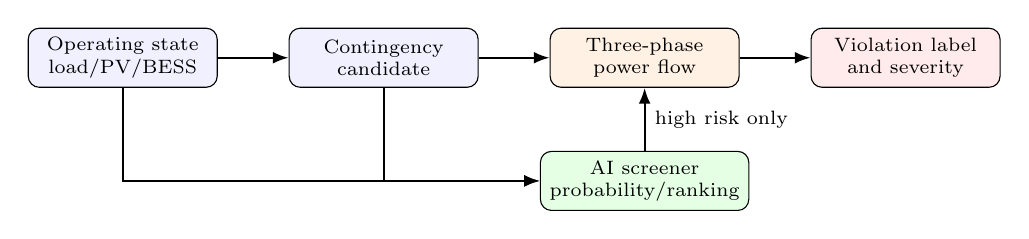
\begin{tikzpicture}[node distance=0.8cm and 0.9cm, every node/.style={font=\scriptsize}]
\tikzset{box/.style={draw, rounded corners, align=center, minimum width=2.4cm, minimum height=0.75cm, fill=blue!6}}
\tikzset{arrow/.style={-{Latex[length=2mm]}, thick}}
\node[box] (state) {Operating state\\load/PV/BESS};
\node[box, right=of state] (cont) {Contingency\\candidate};
\node[box, right=of cont, fill=orange!10] (pf) {Three-phase\\power flow};
\node[box, right=of pf, fill=red!8] (label) {Violation label\\and severity};
\node[box, below=of pf, fill=green!10] (ai) {AI screener\\probability/ranking};
\draw[arrow] (state) -- (cont);
\draw[arrow] (cont) -- (pf);
\draw[arrow] (pf) -- (label);
\draw[arrow] (state) |- (ai);
\draw[arrow] (cont) |- (ai);
\draw[arrow] (ai) -- node[right]{high risk only} (pf);
\end{tikzpicture}
\vspace{0.8em}
\begin{block}{研究问题}
能否用 physics-informed AI 减少大量三相 N-1 潮流调用?
\end{block}
\end{frame}

% ----------------------------------------------------------------------
\begin{frame}{为什么低压 microgrid 要看三相不平衡?}
\begin{itemize}
  \item 单相负荷和单相 PV 可能只接在 A/B/C 中某一相;
  \item EV 充电桩和家用设备的相别分布不均匀;
  \item 线路阻抗、接地方式、变压器接线组会影响零序和负序分量;
  \item 一个 bus 的平均电压安全, 不代表每一相都安全;
  \item N-1 后某一相可能先发生 undervoltage 或 overloading。
\end{itemize}
\begin{block}{Week 1 的处理}
先用 balanced \code{runpp} 学会数据结构和验证方法; Week 2 再把同一思路推广到 phase-aware \code{runpp\_3ph}。
\end{block}
\end{frame}

% ----------------------------------------------------------------------
\begin{frame}{本周先解决的最小问题}
\begin{equation*}
\text{Given a base-case microgrid model } G, \quad \text{compute } V_i, I_\ell, S_\ell.
\end{equation*}
\begin{block}{安全摘要}
\begin{align*}
V_{\min} &= \min_i |V_i|, \\
V_{\max} &= \max_i |V_i|, \\
L_{\max} &= \max_\ell \text{loading}_\ell, \\
y_{N0} &= \mathbb{I}\left(V_{\min}<0.95 \;\vee\; V_{\max}>1.05 \;\vee\; L_{\max}>100\%\right).
\end{align*}
\end{block}
\begin{alertblock}{后续推广}
Week 4 会把 $y_{N0}$ 推广成 $y(x_t,c)$: 某个运行场景 $x_t$ 在 contingency $c$ 后是否 violation。
\end{alertblock}
\end{frame}

% ----------------------------------------------------------------------
\begin{frame}{为什么选 pandapower?}
\begin{columns}[T]
\column{0.52\textwidth}
\begin{itemize}
  \item Python 原生, 适合 Jupyter 教学和科研复现;
  \item 网络对象由 DataFrame 风格的输入表和结果表组成;
  \item 支持 power flow, OPF, contingency analysis, time series 等;
  \item 支持三相/不对称潮流入口 \code{runpp\_3ph};
  \item 便于与 pandas, PyTorch, PyTorch Geometric 连接。
\end{itemize}
\column{0.42\textwidth}
\begin{block}{官方最小流程}
\code{create\_empty\_network} $\rightarrow$ 创建设备 $\rightarrow$ \code{pp.runpp(net)} $\rightarrow$ 查看 \code{net.res\_bus.vm\_pu} 和 \code{net.res\_line.loading\_percent}。
\end{block}
\footnotesize pandapower 官方网站给出了上述入门流程, 并说明其是面向电力系统建模、分析和优化的开源工具。\footnote{pandapower official website, accessed 2026.}
\end{columns}
\end{frame}

% ----------------------------------------------------------------------
\begin{frame}{pandapower 的数据模型}
\centering
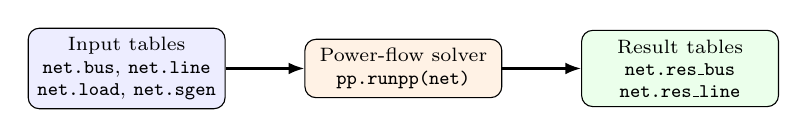
\begin{tikzpicture}[node distance=0.75cm and 1.0cm, every node/.style={font=\scriptsize}]
\tikzset{box/.style={draw, rounded corners, align=center, minimum width=2.5cm, minimum height=0.72cm}}
\node[box, fill=blue!7] (input) {Input tables\\\code{net.bus}, \code{net.line}\\\code{net.load}, \code{net.sgen}};
\node[box, fill=orange!10, right=of input] (solver) {Power-flow solver\\\code{pp.runpp(net)}};
\node[box, fill=green!8, right=of solver] (result) {Result tables\\\code{net.res\_bus}\\\code{net.res\_line}};
\draw[-{Latex[length=2mm]}, thick] (input) -- (solver);
\draw[-{Latex[length=2mm]}, thick] (solver) -- (result);
\end{tikzpicture}
\vspace{1em}
\begin{columns}[T]
\column{0.48\textwidth}
\begin{block}{输入表}
描述设备参数和运行设定值, 例如 bus 电压等级、line 阻抗、load P/Q、PV P/Q。
\end{block}
\column{0.48\textwidth}
\begin{block}{结果表}
潮流收敛后自动填充, 例如 bus voltage, line current, line loading, transformer loading。
\end{block}
\end{columns}
\end{frame}

% ----------------------------------------------------------------------
\begin{frame}[fragile]{最小 pandapower 工作流}
\begin{lstlisting}
import pandapower as pp

net = pp.create_empty_network()
b1 = pp.create_bus(net, vn_kv=20.0, name="grid")
b2 = pp.create_bus(net, vn_kv=20.0, name="load bus")

pp.create_ext_grid(net, bus=b1, vm_pu=1.0)
pp.create_line_from_parameters(
    net, b1, b2, length_km=1.0,
    r_ohm_per_km=0.2, x_ohm_per_km=0.1,
    c_nf_per_km=0.0, max_i_ka=0.4
)
pp.create_load(net, bus=b2, p_mw=1.0, q_mvar=0.2)

pp.runpp(net)
print(net.res_bus.vm_pu)
print(net.res_line.loading_percent)
\end{lstlisting}
\begin{alertblock}{本课程要求}
不要只看代码是否运行, 还要证明结果满足网络结构、功率平衡、线路 loading 公式和跨求解器一致性检查。
\end{alertblock}
\end{frame}

% ----------------------------------------------------------------------
\begin{frame}{Week 1 示例系统}
\begin{columns}[T]
\column{0.48\textwidth}
\begin{itemize}
  \item 20 kV utility grid;
  \item 20 kV PCC / MV bus;
  \item 20/0.4 kV distribution transformer;
  \item 0.4 kV radial LV feeder;
  \item EV load, flexible building load, critical load;
  \item rooftop PV;
  \item battery energy storage system。
\end{itemize}
\column{0.48\textwidth}
\begin{block}{为什么这个系统适合 Week 1?}
\begin{itemize}
  \item 小到足够手算和 debug;
  \item 有微电网故事里的关键对象;
  \item radial topology 便于 NR 和 BFSW 交叉验证;
  \item 后续可以自然扩展到三相和 N-1。
\end{itemize}
\end{block}
\end{columns}
\end{frame}

% ----------------------------------------------------------------------
\begin{frame}{Week 1 系统拓扑}
\centering
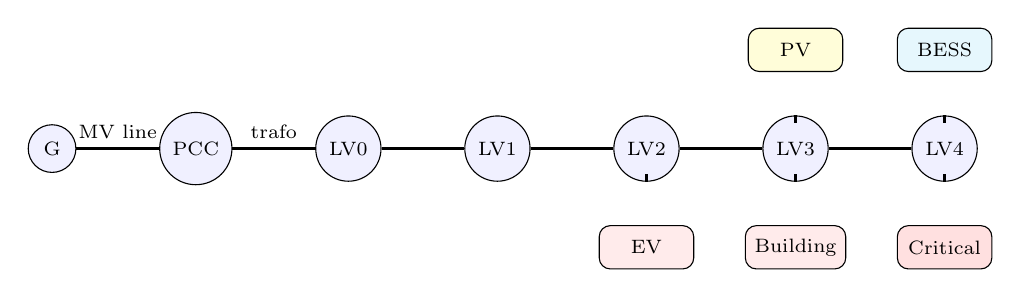
\begin{tikzpicture}[node distance=1.0cm and 1.05cm, every node/.style={font=\scriptsize}]
\tikzset{bus/.style={draw, circle, minimum size=0.5cm, fill=blue!6}}
\tikzset{dev/.style={draw, rounded corners, align=center, minimum width=1.2cm, minimum height=0.55cm}}
\node[bus] (g) {G};
\node[bus, right=of g] (p) {PCC};
\node[bus, right=of p] (l0) {LV0};
\node[bus, right=of l0] (l1) {LV1};
\node[bus, right=of l1] (l2) {LV2};
\node[bus, right=of l2] (l3) {LV3};
\node[bus, right=of l3] (l4) {LV4};
\draw[thick] (g) -- node[above]{MV line} (p);
\draw[thick] (p) -- node[above]{trafo} (l0);
\draw[thick] (l0) -- (l1) -- (l2) -- (l3) -- (l4);
\node[dev, below=0.55cm of l2, fill=red!8] {EV};
\node[dev, below=0.55cm of l3, fill=red!8] {Building};
\node[dev, below=0.55cm of l4, fill=red!12] {Critical};
\node[dev, above=0.55cm of l3, fill=yellow!15] {PV};
\node[dev, above=0.55cm of l4, fill=cyan!10] {BESS};
\draw[thick] (l2) -- ++(0,-0.32);
\draw[thick] (l3) -- ++(0,-0.32);
\draw[thick] (l4) -- ++(0,-0.32);
\draw[thick] (l3) -- ++(0,0.32);
\draw[thick] (l4) -- ++(0,0.32);
\end{tikzpicture}
\vspace{0.6em}
\small 这个系统不是真实工程参数库, 而是教学用的可解释、可验证 benchmark。
\end{frame}

% ----------------------------------------------------------------------
\begin{frame}{符号约定: load, sgen, storage}
\begin{table}
\centering
\small
\begin{tabular}{lll}
\toprule
元素 & 正的 $P$ 代表什么? & Week 1 解释 \\
\midrule
\code{load} & 消耗有功功率 & 普通负荷, EV, critical load \\
\code{sgen} & 注入有功功率 & rooftop PV 或 inverter-based DER \\
\code{storage} & 充电消耗有功功率 & $p>0$ 充电, $p<0$ 放电 \\
\code{ext\_grid} & 与上级电网交换功率 & 正值通常表示从上级电网进口 \\
\bottomrule
\end{tabular}
\end{table}
\begin{alertblock}{重点}
pandapower storage 文档明确说明: \code{p\_mw} 正值为 charging, 负值为 discharging; SOC 不会在默认潮流计算中自动更新。\footnote{pandapower storage documentation, accessed July 2026.}
\end{alertblock}
\end{frame}

% ----------------------------------------------------------------------
\begin{frame}{静态安全检查: Week 1 版本}
\begin{columns}[T]
\column{0.48\textwidth}
\begin{block}{Voltage check}
\begin{equation*}
0.95 \le V_i \le 1.05, \quad \forall i
\end{equation*}
常用作教学阈值, 实际工程阈值应由标准、规划准则或项目要求决定。
\end{block}
\column{0.48\textwidth}
\begin{block}{Thermal check}
\begin{equation*}
\text{loading}_\ell \le 100\%, \quad \forall \ell
\end{equation*}
这里的 loading 来自线路电流与额定电流的比值。
\end{block}
\end{columns}
\vspace{0.8em}
\begin{alertblock}{重要转折}
Week 2 之后, 所有检查都会变成 phase-aware: $V_{i,a},V_{i,b},V_{i,c}$ 和 $I_{\ell,a},I_{\ell,b},I_{\ell,c}$。
\end{alertblock}
\end{frame}

% ----------------------------------------------------------------------
\begin{frame}[fragile]{Proof 1: 网络结构检查}
\begin{lstlisting}
def validate_network_structure(net):
    assert len(net.bus) == 7
    assert len(net.line) == 5
    assert len(net.trafo) == 1
    assert len(net.ext_grid) == 1
    assert (net.bus.vn_kv > 0).all()
    assert (net.line.length_km > 0).all()
    assert (net.line.max_i_ka > 0).all()

    # Build a graph with line and transformer edges.
    # Every bus must be reachable from the external grid.
    # The Week 1 network is intentionally radial.
\end{lstlisting}
\begin{block}{目的}
很多潮流错误不是算法问题, 而是输入数据问题: 孤立 bus, 错电压等级, 额定电流缺失, 或拓扑不连通。
\end{block}
\end{frame}

% ----------------------------------------------------------------------
\begin{frame}[fragile]{Proof 2: 功率平衡检查}
\begin{lstlisting}
p_expected_ext = (
    p_load + p_storage - p_sgen
    + p_line_loss + p_trafo_loss
)
p_residual = p_ext - p_expected_ext
assert abs(p_residual) <= 1e-5
\end{lstlisting}
\begin{block}{物理含义}
外部电网进口功率应等于: 负荷 + BESS 充电 - PV 注入 + line/trafo 损耗。若 BESS 放电, \code{p\_storage} 为负, 会降低外部电网进口。
\end{block}
\begin{alertblock}{注意}
这不是替代潮流方程求解, 而是结果表级别的全局守恒 audit。
\end{alertblock}
\end{frame}

% ----------------------------------------------------------------------
\begin{frame}[fragile]{Proof 3: line loading 手算复核}
\begin{lstlisting}
i_limit = net.line.max_i_ka * net.line.df * net.line.parallel
i_terminal = max(abs(i_from_ka), abs(i_to_ka))
manual_loading = 100 * i_terminal / i_limit

assert abs(manual_loading - net.res_line.loading_percent) < tol
\end{lstlisting}
\begin{block}{为什么要这样做?}
\code{loading\_percent} 是可以从电流和额定值复核的工程量。
\end{block}
\end{frame}

% ----------------------------------------------------------------------
\begin{frame}[fragile]{Proof 4: 跨求解器交叉验证}
\begin{lstlisting}
nr_net = copy.deepcopy(net)
bfsw_net = copy.deepcopy(net)

run_balanced_pf(nr_net, algorithm="nr")
run_balanced_pf(bfsw_net, algorithm="bfsw")

vm_diff = max(abs(nr_net.res_bus.vm_pu - bfsw_net.res_bus.vm_pu))
loading_diff = max(abs(nr_net.res_line.loading_percent
                       - bfsw_net.res_line.loading_percent))
assert vm_diff <= 2e-3
assert loading_diff <= 1.0
\end{lstlisting}
\begin{block}{解释}
对这个 radial feeder, Newton-Raphson 和 backward/forward sweep 应给出接近结果。若差异很大, 优先检查网络数据和 solver 设置。
\end{block}
\end{frame}

% ----------------------------------------------------------------------
\begin{frame}{Week 1 场景设计}
\begin{table}
\centering
\scriptsize
\begin{tabular}{lccccl}
\toprule
Scenario & Load scale & PV scale & BESS $P$ & 预期现象 & 用途 \\
\midrule
base & 1.00 & 1.00 & 0.000 & 正常运行 & 基准 \\
morning\_low\_pv & 0.75 & 0.30 & 0.000 & 低负荷低 PV & 对照 \\
noon\_high\_pv & 0.80 & 2.00 & 0.000 & PV 高出力 & 反向潮流入门 \\
evening\_peak\_bess\_discharge & 1.35 & 0.00 & -0.040 & 晚高峰放电 & BESS 支撑 \\
bess\_charging\_peak & 1.25 & 0.20 & 0.050 & 高负荷充电 & 电压下降 \\
stress\_high\_load\_charging & 2.00 & 0.00 & 0.040 & 压力测试 & violation 示例 \\
\bottomrule
\end{tabular}
\end{table}
\begin{alertblock}{讨论}
为什么 BESS 充电可能比 PV 停发更危险? 为什么高 PV 有时会改善电压, 有时也可能导致过电压?
\end{alertblock}
\end{frame}

% ----------------------------------------------------------------------
\begin{frame}{Notebook 输出: security summary}
\begin{table}
\centering
\scriptsize
\begin{tabular}{lrrrr}
\toprule
Scenario & Grid import MW & Min $V$ pu & Max loading \% & Violation? \\
\midrule
base & 0.064 & 0.979 & 33.2 & False \\
noon high PV & 0.014 & 1.009 & 13.5 & False \\
evening peak + discharge & 0.087 & 0.971 & 45.5 & False \\
BESS charging peak & 0.175 & 0.905 & 84.7 & True \\
stress high load + charging & 0.258 & 0.854 & 126.2 & True \\
\bottomrule
\end{tabular}
\end{table}
\begin{block}{解释}
这些数值来自 Notebook 的可复现实验。学生运行时应关注趋势, 而不只是记住数值。
\end{block}
\end{frame}

% ----------------------------------------------------------------------
\begin{frame}{如何把 Week 1 连接到论文?}
\begin{columns}[T]
\column{0.5\textwidth}
\begin{block}{Week 1 产出}
\begin{itemize}
  \item 一个可运行的 pandapower network;
  \item base-case static security summary;
  \item validation and audit functions;
  \item scenario table;
  \item 初步图表和解释。
\end{itemize}
\end{block}
\column{0.45\textwidth}
\begin{block}{论文中的位置}
这些内容会进入:
\begin{itemize}
  \item dataset generation pipeline;
  \item simulation validation;
  \item security label definition;
  \item reproducibility section。
\end{itemize}
\end{block}
\end{columns}
\end{frame}

% ----------------------------------------------------------------------
\begin{frame}{常见建模错误}
\begin{enumerate}
  \item \warnitem 只创建 bus, 忘记 ext\_grid 或 slack source;
  \item \warnitem line 的 from\_bus/to\_bus 接错, 造成孤立节点;
  \item \warnitem 20 kV 和 0.4 kV bus 直接用 line 连接, 忘记 transformer;
  \item \warnitem 把 storage 的正负号理解反了;
  \item \warnitem 只看平均电压, 不看最差 bus;
  \item \warnitem 没检查 \code{net.converged};
  \item \warnitem scenario loop 直接修改原始网络, 结果互相污染;
  \item \warnitem 用 Week 1 balanced 结果声称已完成三相不平衡安全分析。
\end{enumerate}
\end{frame}

% ----------------------------------------------------------------------
\begin{frame}{课堂 walkthrough 建议}
\begin{enumerate}
  \item 先画出 physical topology, 再展示 pandapower 表;
  \item 从 \code{net.bus} 和 \code{net.line} 开始, 不急着运行潮流;
  \item 运行 base case 后先问: 哪个 bus 电压最低? 哪条线 loading 最高?;
  \item 解释 PV 和 BESS 对 grid import 的影响;
  \item 展示 proof cells: 结构检查、功率平衡、loading 复核、跨求解器验证;
  \item 最后运行 scenario suite, 引出 Week 2/3/4。
\end{enumerate}
\end{frame}

% ----------------------------------------------------------------------
\begin{frame}{讨论问题}
\begin{itemize}
  \item 如果只能监视 3 个变量, 选择哪些变量作为安全预测特征?
  \item 哪个 scenario 最危险? 危险来自 voltage 还是 thermal loading?
  \item BESS 放电为什么可能降低 grid import, 但不一定消除 voltage violation?
  \item 高 PV 场景下, grid import 可能变小甚至变负, 这对保护和电压控制意味着什么?
  \item 为什么 AI screening 比 accuracy 更关键?
\end{itemize}
\end{frame}

% ----------------------------------------------------------------------
\begin{frame}{Homework}
\begin{block}{必做}
\begin{enumerate}
  \item 运行完整 Notebook 1;
  \item 修改 PV scale 和 load scale, 找到一个新的 undervoltage 场景;
  \item 保留所有 proof cells 通过;
  \item 写 5-8 句话解释最危险 scenario 的物理原因。
\end{enumerate}
\end{block}
\begin{block}{选做}
\begin{enumerate}
  \item 增加一个新的 BESS setpoint scenario;
  \item 把 voltage limit 从 0.95/1.05 改成更严格阈值, 比较 violation flags;
  \item 记录 grid import 与 min voltage 的关系。
\end{enumerate}
\end{block}
\end{frame}

% ----------------------------------------------------------------------
\begin{frame}{Week 2 预告}
\begin{columns}[T]
\column{0.48\textwidth}
Week 2 会把本周模型升级为三相不平衡模型:
\begin{itemize}
  \item \code{asymmetric\_load};
  \item \code{asymmetric\_sgen};
  \item line zero-sequence parameters;
  \item \code{runpp\_3ph};
  \item \code{res\_bus\_3ph}, \code{res\_line\_3ph};
  \item voltage unbalance factor。
\end{itemize}
\column{0.48\textwidth}
\begin{alertblock}{连接点}
Week 1 的验证方法仍然有效, 但所有检查都会变成 phase-aware: 不能只检查平均电压或总 loading。
\end{alertblock}
\footnotesize pandapower 文档说明 \code{runpp\_3ph} 用 sequence frame 求解三相潮流, 正序网络使用 NR, 零序和负序网络使用 current injection 方法。\footnote{pandapower asymmetric / three-phase power-flow documentation, accessed July 2026.}
\end{columns}
\end{frame}


% ----------------------------------------------------------------------
\begin{frame}{References and documentation}
\footnotesize
\begin{itemize}
  \item DOE Grid Deployment Office, \emph{Microgrid Overview Fact Sheet}, 2024.
  \item pandapower official website, \emph{Getting started example and overview}, accessed 2026.
  \item pandapower documentation, \emph{Balanced AC Power Flow}, accessed July 2026.
  \item pandapower documentation, \emph{Storage element}, accessed July 2026.
  \item pandapower documentation, \emph{Asymmetric / Three Phase Power Flow}, accessed July 2026.
\end{itemize}
\vspace{0.8em}
\begin{block}{材料使用建议}
本课件与 Notebook 1 配套使用。课堂中重点运行、修改、解释和验证知识点。
\end{block}
\end{frame}

\end{document}
